\section{Building block view}
UML package and class diagrams (perhaps auto-generate with tool, but ensure clean and well-organized)
Include description of responsibility and name of each package and class.
List external software used and provide links


\subsection{Games Importer Service}
\subsubsection{Class Diagrams}
\graphic{GamesImporter}{Klassendiagramm des Game Importer Service}
\subsubsection{Responsibilities}
Dieser Service ist dafür zuständig, die benötigten Daten bei der Riot API anzufragen und dann in der LoL Datenbank zu speichern. Die Struktur des Services ist im obigen Klassendiagramm zu sehen. \\
Die db Klasse bietet alle Funktionen, um mit der Datenbank zu interagieren: neue Daten speichern, Daten lesen und Daten updaten. Dazu wird das psycopg2 Package verwendet.\\
Die App Klasse beinhaltet den main loop (update\_loop Funktion). In dieser werden dann weitere Funktionen aufgerufen, um alle Spieler zu updaten. Dazu werden zuerst die Methoden des summoner.py Moduls verwendet, welche einen einzelnen Spieler updaten können. In dieser Methode werden zunächst alle Daten des Summoners (Level, Name, ...) aktualisiert. Dann wird das matchhistory.py Modul verwendet, welches für den Spieler die MatchHistory importieren kann (add\_missing\_games\_tp\_db(db, get\_match\_ids(), puuid). Dieses verwendet dabei noch die Challenges Klasse, welche die Challenges für einzelne Spieler speichern kann (store\_challenges()). Dabei werden mithilfe der in der Datenbank vorhandenen Werte für total, average und highscore die neuen Werte berechnet und diese dann gespeichert.\\

Der PlayerImportRequest erbt von der von GRPC generierten Klasse ImporterService und ist für die Verbindung mit der PlayerAPI zuständig. Über diese Klasse kann eine Anfrage gesendet werden, um den Import eines neuen Spielers zu starten, wobei dann dieselbe Abfolge durchlaufen wird wie oben bereits beim updaten eines Spielers beschrieben.

\subsubsection{External Software}
GRPC: \href{https://grpc.io/docs/languages/python/basics/}\\
Cassiopeia: \href{https://github.com/meraki-analytics/cassiopeia}\\
Riot Watcher: \href{https://github.com/pseudonym117/Riot-Watcher}\\
psycopg2: \href{https://pypi.org/project/psycopg2/}\\
Riot API: \href{https://developer.riotgames.com/}\\

\subsection{Player API}
\subsubsection{Class Diagrams}
\subsubsection{Responsibilities}
\subsubsection{External Software}
\subsection{User Management}
\subsubsection{Class Diagrams}
\subsubsection{Responsibilities}
\subsubsection{External Software}


\subsection{Frontend}

\subsubsection{Mockups}

\begin{figure}
\centering
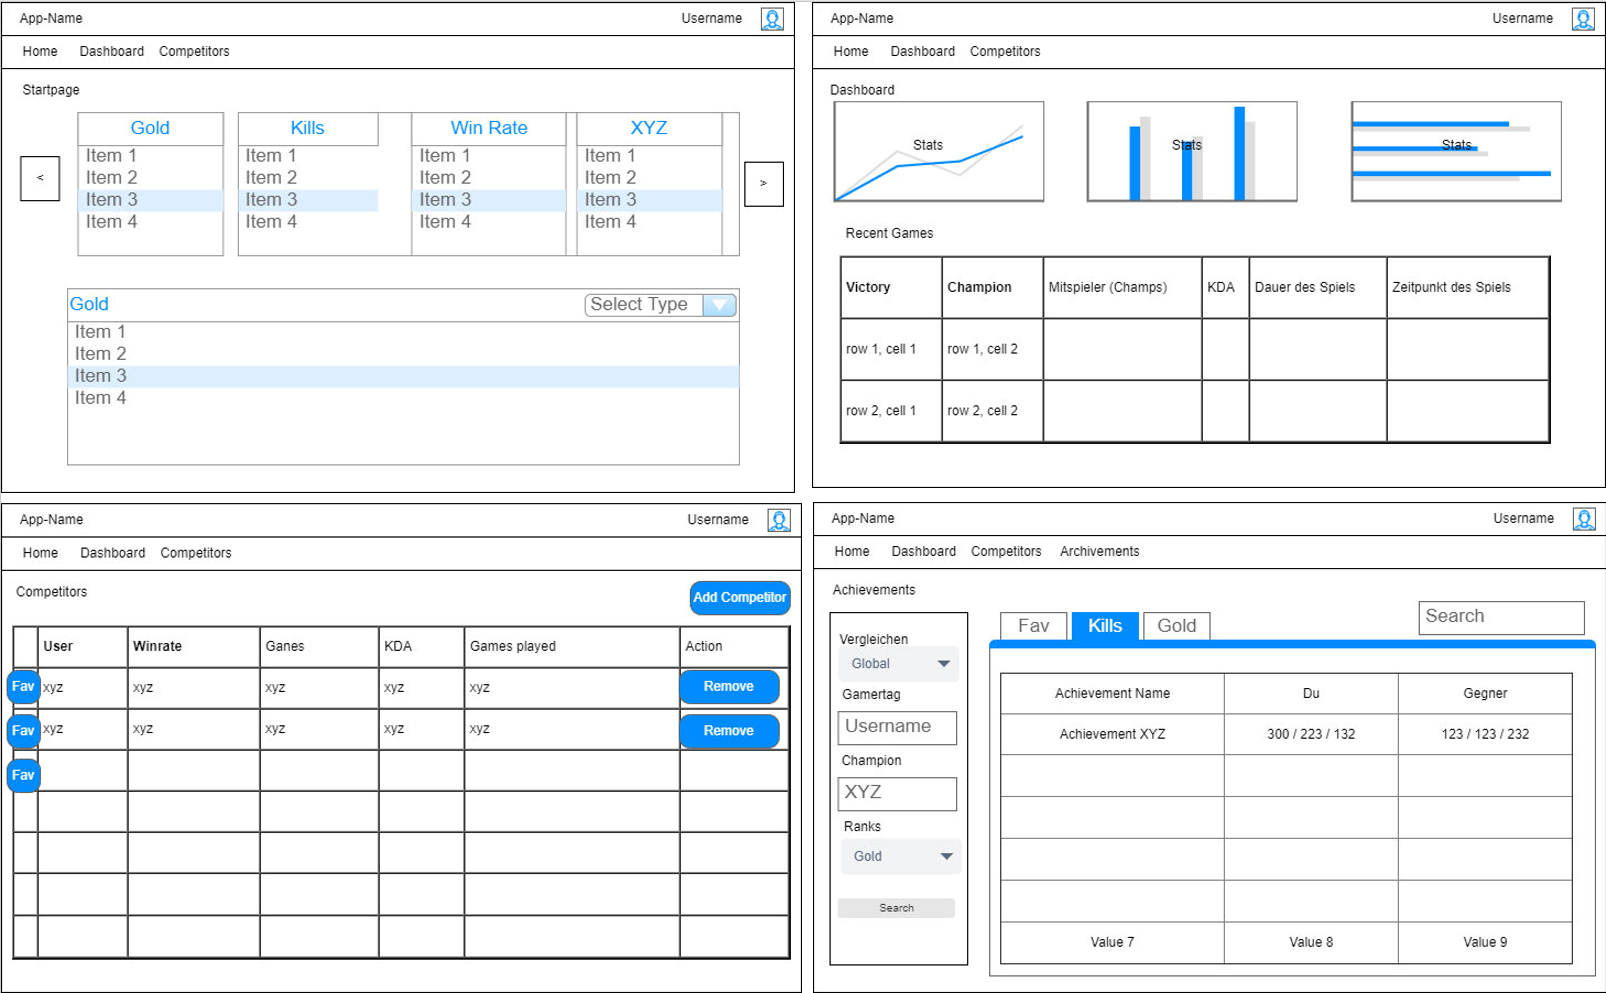
\includegraphics[width=1\textwidth]{mockups/mockup_all.png}
\caption{Alle Mockups des Frontends}
\label{fig:mockups_dashboard}
\end{figure}

\subsubsection{Responsibilities}
Die Benutzeroberfläche (Frontend) dient als Client und ist für die Kommunikation mit dem verschiedenen Microservices zuständig. Es stellt die Daten übersichtlich dar und sorgt für eine
angenehmes Nutzererlebnis.

\subsubsection{External Software}